\begin{frame}{Biological Analogy}
    \begin{figure}[H]
		\centering
		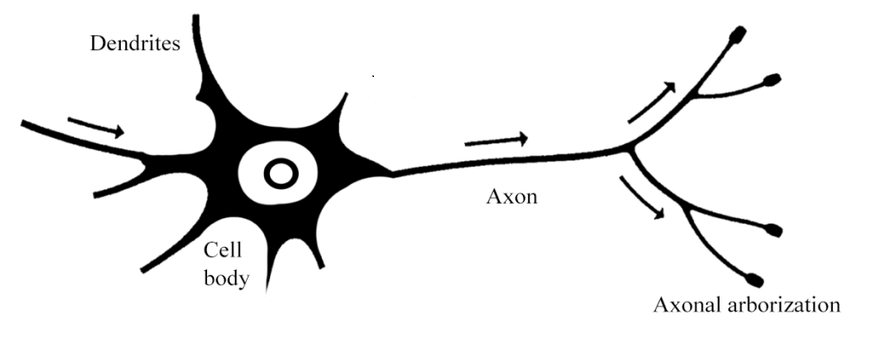
\includegraphics[width=0.9\textwidth]{Images/biological_neuron.png}
		\caption{Anatomy of a biological neuron \cite{biological-and-nn-neuron}.}
	\end{figure}
\end{frame}

\begin{frame}{Biological analogy}
    \begin{figure}[H]
		\centering
		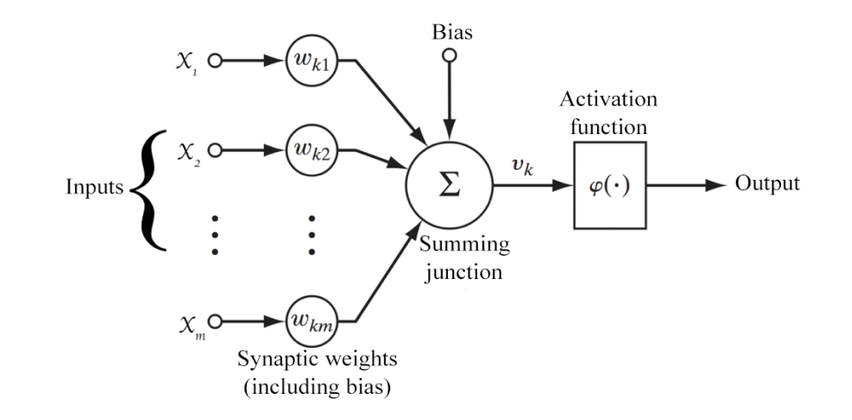
\includegraphics[width=0.9\textwidth]{Images/nn_neuron.png}
		\caption{Neural network neuron \cite{biological-and-nn-neuron}.}
	\end{figure}
\end{frame}

\begin{frame}{Activation Functions}
    \begin{figure}[H]
		\centering
		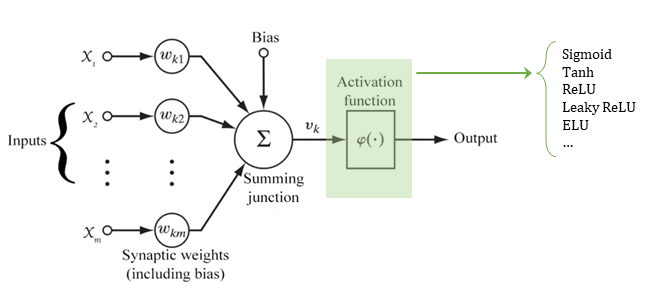
\includegraphics[width=0.9\textwidth]{Images/activation_function_1.png}
		\caption{Activation function}
	\end{figure}
\end{frame}

\begin{frame}{Activation Functions}
    \begin{figure}[H]
		\centering
		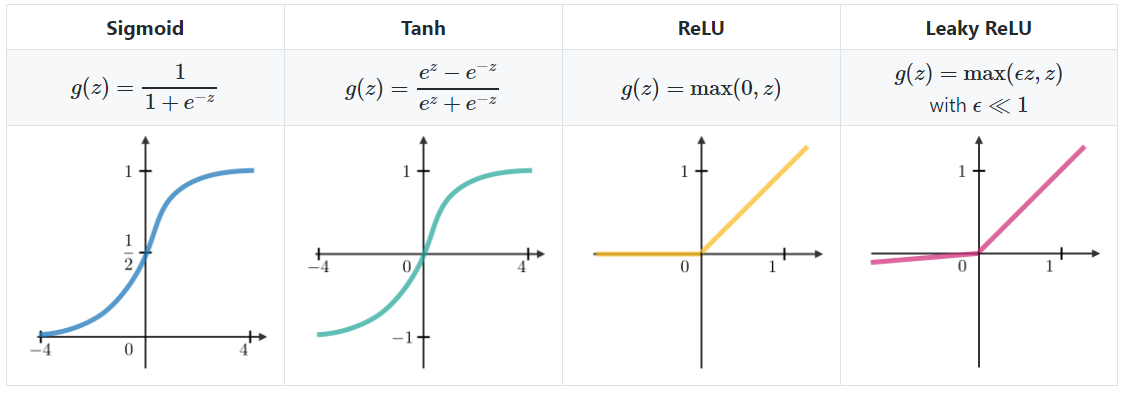
\includegraphics[width=0.9\textwidth]{Images/activation_function_2.png}
		\caption{Activation functions \cite{activation-functions}.}
	\end{figure}
\end{frame}

\begin{frame}{Gradient Descent}
    \begin{figure}[H]
		\centering
		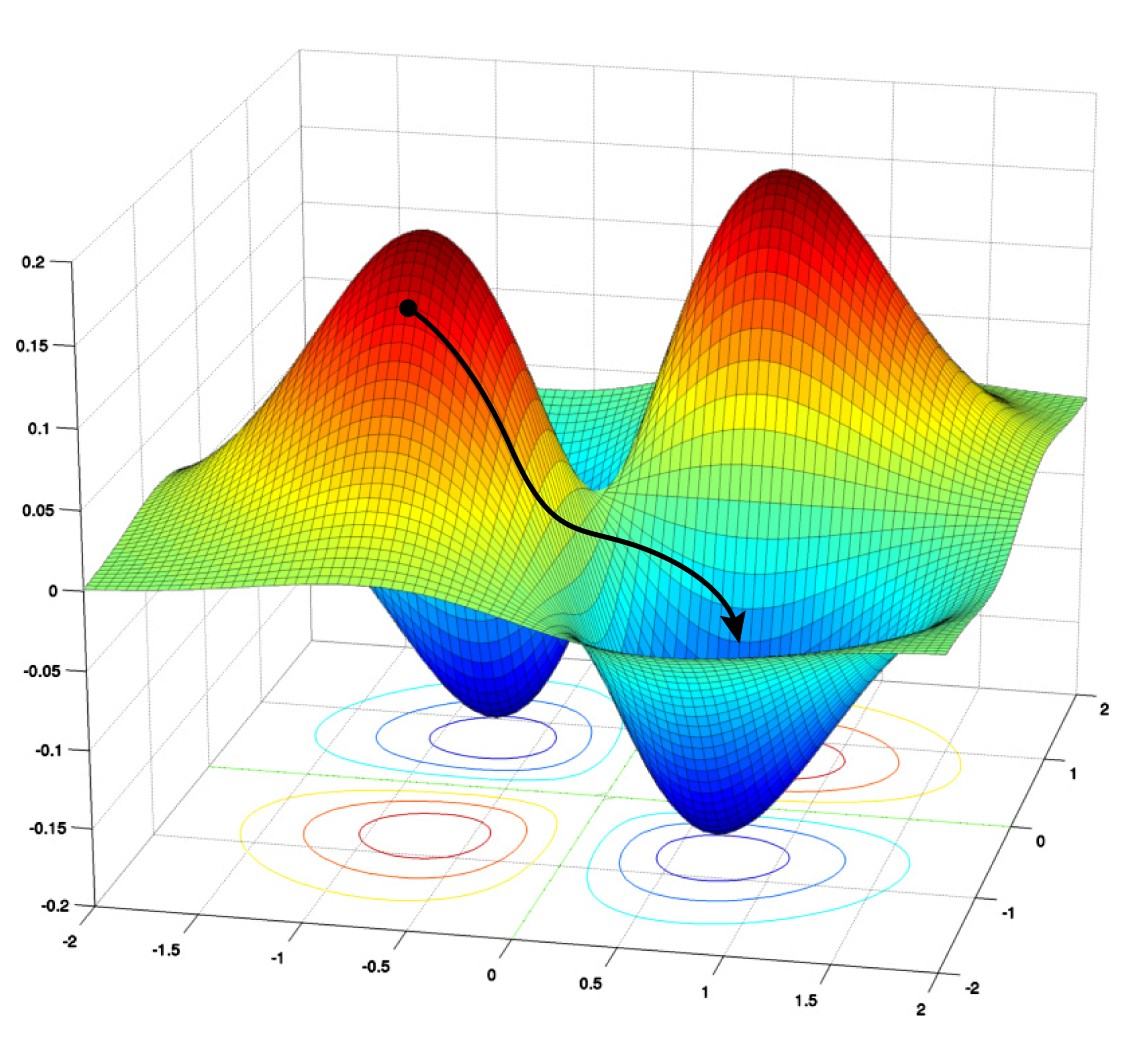
\includegraphics[width=0.5\textwidth]{Images/gradient_descent.jpg}
		\caption{Gradient descent \cite{gradient-descend}.}
	\end{figure}
\end{frame}





